\chapter{Methodology}

In this chapter, we describe the methodology of our proposed Android malware detection system based on static features and how we implemented our models using our proposed Stacking method.

\section{Dataset} \label{dataset}

To begin with this Chapter we will introduce the dataset used in this paper. We used a dataset called Androzoo.
AndroZoo is a growing collection of Android Applications collected from several sources, including the official Google Play app market.
It currently contains 10,299,119 different APKs, each of which has been (or will soon be) analyzed by tens of different AntiVirus products to know which applications are detected as Malware\cite{androzoo}.

Due to keeping a balanced dataset containing both malware and benignware samples,
We collected 10,000 malware \ac{apk}s and 10,000 benignware samples randomly from the above dataset Androzoo. Also, we have done a filtering process in which we remove repeated applications and those that are considered as invalid (they cannot be actually installed and executed). After removing these applications we download again the remaining number to complete 10,000 of \ac{apk}s and done the filtering process again. We repeated these steps until to gather a clean dataset consisted of 10,000 \ac{apk}s of malware applications and 10,000 \ac{apk}s of benignware applications with a total of 20,000 \ac{apk}s.

\section{Static Features extraction} \label{extractedvector}

Static features focus on a large part of the state-of-the-art literature related to Android malware
detection. The easy and quick extraction of this kind of feature makes them suitable to be used to build malware detection tools.

One of our system goals is to do a prediction process while the user only needs to input the \ac{apk} file to receive the output (malware or not). In other words, it is called an end-to-end system. One essential process to achieve this goal is, we have to automatically the feature extraction process and convert it to vectors that the machine learning models could use for inputs to predict something.
So in this study, we use an opensource tool called AndroPytool \cite{andropytool}.

AndroPyTool can extract static and dynamic features, this section focuses on the
former ones. By using Android malware analysis tools such as AndroGuard or by analyzing the source code of each sample, AndroPyTool extracts a representative set of characteristics based on state-of-the-art Android malware detection approaches. These features include API calls, main activity name, opcodes, package name, permissions, intent receivers, intents services, intent activities, strings found, system commands or information flows extracted with FlowDroid.

Once extracted the desired set of characteristics, such as permissions requested, API calls
invoked or information flows, all this information is processed to build a representative feature
vector for each application. This process is shown in Fig. \ref{fig:featurevector} On the one hand, $M$ measurable
characteristics $$ C_{M}=\left\{c_{1}, c_{2}, \ldots, c_{M}\right\} $$ are assigned a value counting the number of occurrences of
that feature within the application. On the other hand, $K$ binary features $$
D_{K}=\left\{d_{1}, d_{2}, \ldots, d_{K}\right\}
$$
point the use or the existence of a particular attribute. The bundling of both features composes
the static description of the application behavior, in other words, our input dataset $\mathcal{D}$.
$$
\mathcal{D}=\left\{\mathbf{x}_{i}, y_{i}\right\} \text{where }
\mathbf{x}_{i}=\left\{c_{1,}^{i} c_{2}^{i}, \ldots, c_{M}^{i}, d_{l,}^{i}, d_{2}^{i}, \ldots, d_{K}^{i}\right\}
$$

\begin{figure}[htbp]
    \centering
    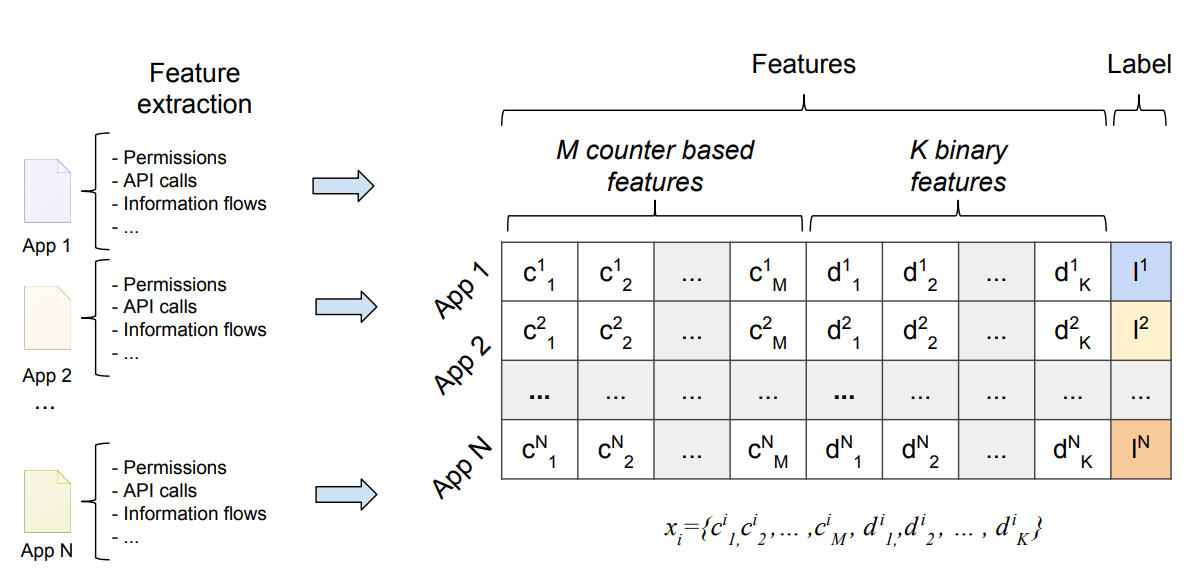
\includegraphics[scale=0.68]{./Figure/featurevector.png}
    \caption{Extraction and representation of static information into representative feature vectors. \cite{andropytool}}
    \label{fig:featurevector}
\end{figure}


\section{Stacking}
Stacking is an ensemble learning technique that combines multiple classifications or regression models via a meta-classifier or a meta-regressor \cite{stackingref}. The base level models are trained based on a complete training set, then the meta-model is trained on the outputs of the base level model like features as we can see in Figure \ref{fig:stacking}.

\begin{figure}[htbp]
    \centering
    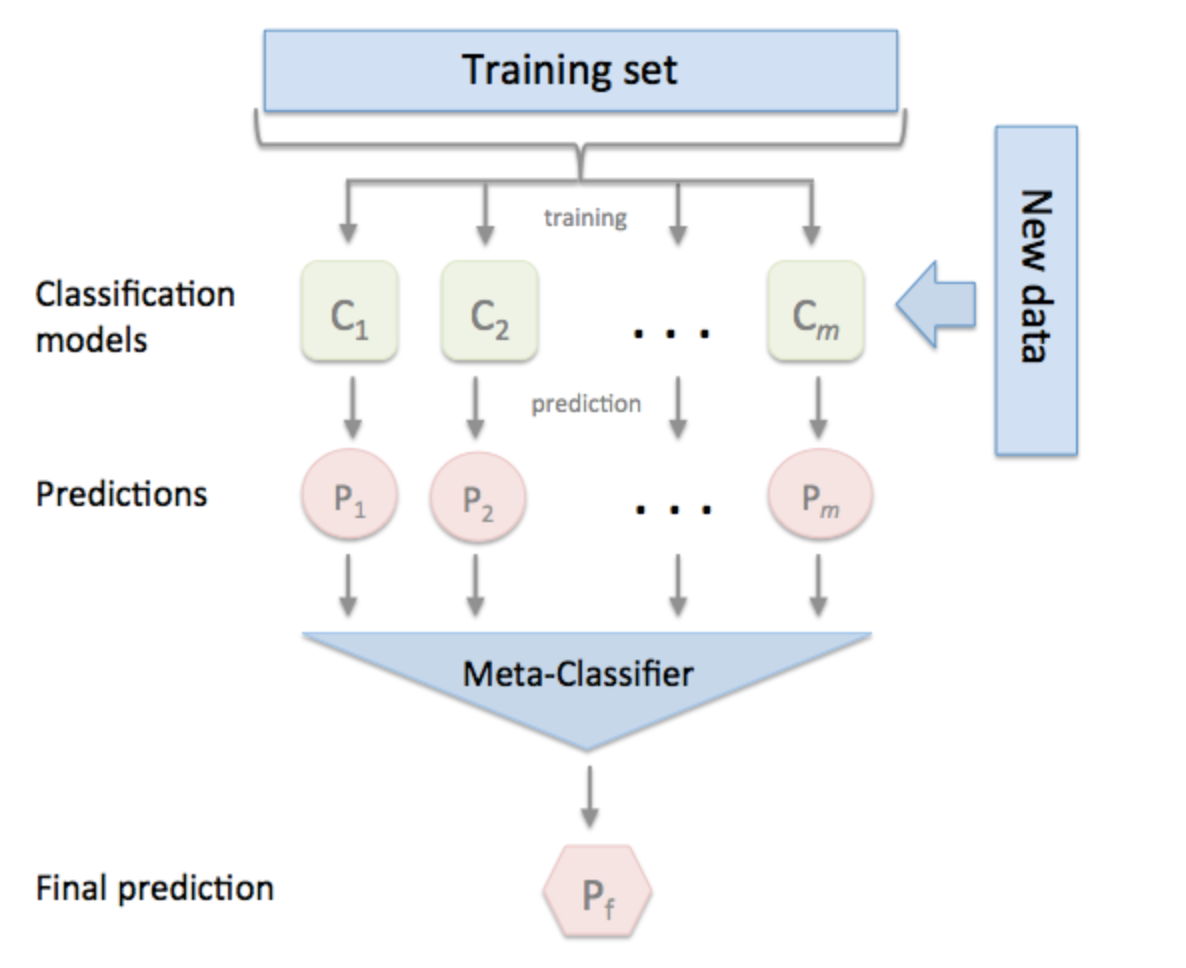
\includegraphics[width=\textwidth]{./Figure/stacking.png}
    \caption{Stacking pipeline figure.}
    \label{fig:stacking}
\end{figure}


The base level often consists of different learning algorithms and therefore stacking ensembles are often heterogeneous. But we must note that this type of Stacking is prone to overfitting due to information leakage. We should not derive the predictions for the 2nd-level classifier from the same dataset that was used for training the level-1 classifiers. The algorithm \ref{alg:algo1} summarizes stacking.

\begin{algorithm}[htbp]
    \centering
    \caption{Stacking}
    \label{alg:algo1}
    \begin{algorithmic}[1]  
    \renewcommand{\algorithmicrequire}{\textbf{Input:}}
    \renewcommand{\algorithmicensure}{\textbf{Output:}}
    \Require Training data $\mathcal{D}=\left\{\mathbf{x}_{i}, y_{i}\right\}_{i=1}^{m}\left(\mathbf{x}_{i} \in \mathbb{R}^{n}, y_{i} \in \mathcal{Y}\right)$
    \Ensure An ensemble classifier $H$
    \State Step 1: Learn first-level classifiers
    \For{$t\gets$ 1 to $T$}
        \Statex Learn a base classifier $h_{t}$ based on $\mathcal{D}$
    \EndFor
    \State Step 2: Construct new data sets from $\mathcal{D}$
    \For{$i = 1$ to $m$}
    \State $\text{Construct a new data set }\mathcal{D}_{h}=\left\{\mathbf{x}_{i}^{\prime}, y_{i}\right\}, \text { where } \mathbf{x}_{i}^{\prime}=\left\{h_{1}\left(\mathbf{x}_{i}\right), \ldots, h_{T}\left(\mathbf{x}_{i}\right)\right\}$
    \EndFor
    \State Step 3: learn a meta-classifier
    \State Learn a new classifier $h^{\prime}$ based on the newly constucted data set $\mathcal{D}_h$
    \State \textbf{return} $H(\mathbf{x})=h^{\prime}\left(\mathcal{D}_h\right)$
    \end{algorithmic}
\end{algorithm}

Besides, Stacking is a commonly used technique for winning the Kaggle data science competition. For example, the first place for the Otto Group Product Classification challenge was won by a stacking ensemble of over 30 models whose output was used as features for three meta-classifiers: XGBoost, Neural Network, and Adaboost.

\section{Proposed model pipeline} \label{model}

In this section, we will introduce our proposed Stacking model pipeline as we can see in Figure\ref{fig:modelpipeline}. Our proposed model consists of 3 stages with different models to predict one final output.

\begin{figure}[htbp]
    \centering
    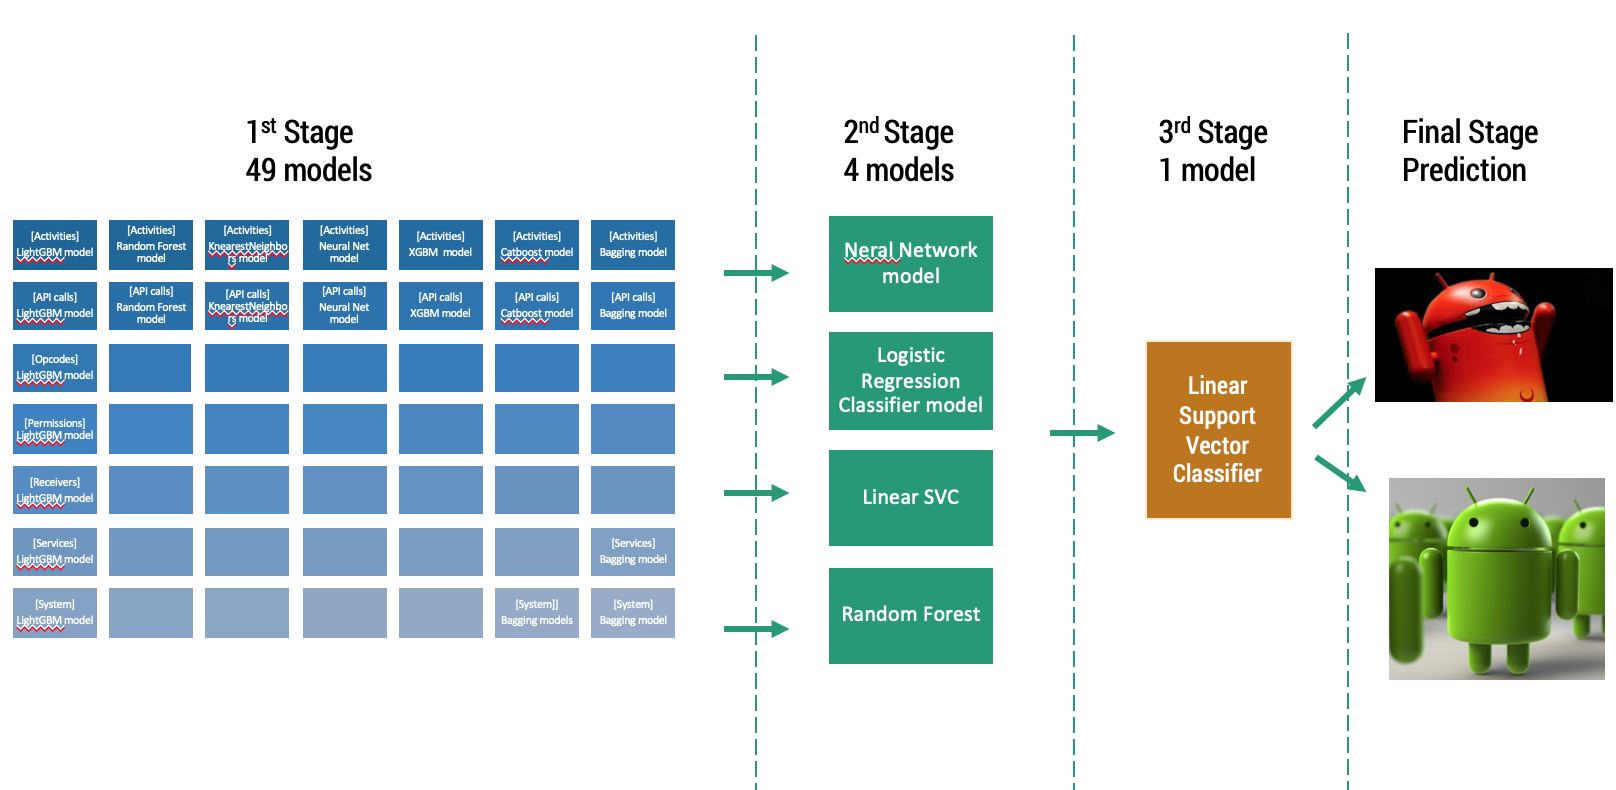
\includegraphics[width=\textwidth]{./Figure/modelpipeline.png}
    \caption{Proposed Stacking model pipeline figure.}
    \label{fig:modelpipeline}
\end{figure}

\subsection{1st Stage}
For this first stage, we proposed to train 7 different algorithms (Bagging, XGBoost, K-neighbors, LogisiticRegression, RandomForest NeuralNetworks) to each 7 different static feature (Activities, API calls, Opcodes, Permissions, Receivers, Services, System commands) to create our models of a total of 49 models. 

Following the Algorithm \ref{alg:algo1}, we trained the base 49 classifiers $h_{t=49}$ on our training dataset as mentioned in section \ref{dataset}. Where our input training data is $\mathbf{x}_{i}$ and label data is $y_{i}$
 $$\left\{\mathbf{x}_{i}, y_{i}\right\}_{i=1}^{m=7}\left(\mathbf{x}_{i} \in \mathbb{R}^{n}, y_{i} \in \mathcal{Y}\right)$$


Due to every model has one output for one \ac{apk} input, we gain one output vector from $\mathcal{D}$ as we can see at below $$\mathcal{D}_h = \left\{\mathbf{x}_{i}^{\prime}, y_{i}\right\}, \text { where } \mathbf{x}_{i}^{\prime}=\left\{h_{1}\left(\mathbf{x}_{i}\right), \ldots, h_{T=49}\left(\mathbf{x}_{i}\right)\right\}$$

\subsection{2nd Stage}
In this stage, we proposed to train 4 different algorithms (Neural Network, Logistic Regression classifier, Linear SVC, RandomForest) with the output vector from the 1st stage as input data.
Following the Algorithm \ref{alg:algo1}, we train our 2nd stage meta-classifiers $H_{k}$($k=4$) based on the newly constructed data set at 1st stage $\mathcal{D}_h$. Then we obtained the below models $H_{k}$
$$H_{k}(\mathbf{x})=h^{\prime}\left(\mathcal{D}_h\right)$$



\subsection{3rd Stage}
In this stage, we repeated the 2nd stage process using $H_{k}\left(\mathbf{x}\right)$ as input to train our final meta-classifier (Linear SVC).

We trained our final meta-classifier $L$ based on the newly constructed dataset at 2nd stage $\mathcal{D}_l = \left\{\mathbf{h}_{i}^{\prime}, y_{i}\right\}$. Then we obtain the below trained final meta-classifier $L\left(\mathbf{x}\right)$
$$L(\mathbf{x})=l^{\prime}\left(H_{1}(\mathbf{x}), H_{2}(\mathbf{x}), \ldots, H_{k}(\mathbf{x})\right)$$



\section{Proposed Malware detection System}
In this section, we introduce our proposed malware detection system implementing our proposed Stacking model in section \ref{model}. We can see the overview of our proposed system pipeline in Figure \ref{fig:systempip}.

\begin{figure}[htbp]
    \centering
    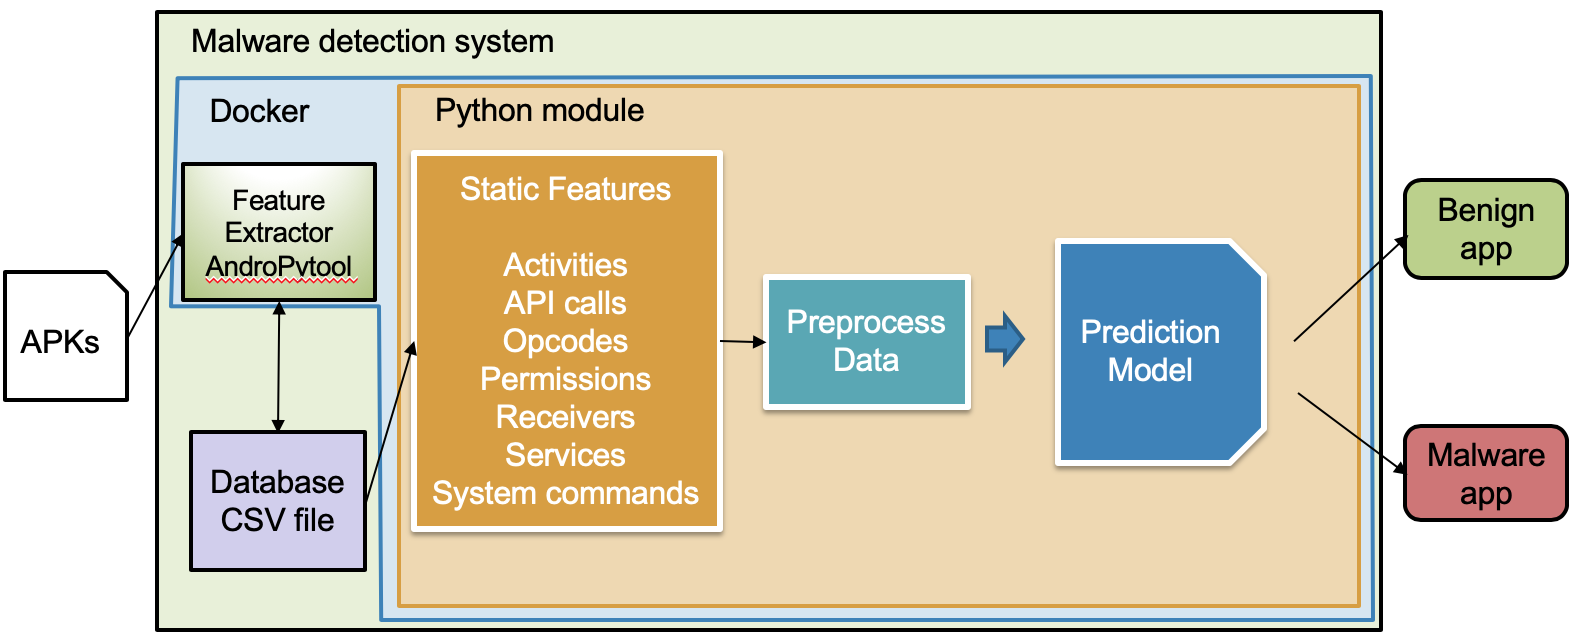
\includegraphics[width=\textwidth]{./Figure/systempip.png}
    \caption{Proposed malware detection system pipeline figure.}
    \label{fig:systempip}
\end{figure}

\subsection{AndroPytool module}

We build almost all of this system in a Linux Docker container. The main merit of building a system with Docker is that it makes easy for the users to deploy this system in other environments not needing to care about dependent packages. 

First, we implemented the AndroPyTool\cite{andropytool} module. Here we input the APK file to extract the static features to our database as \ac{csv} file, as we can see in section \ref{extractedvector}.  

\subsection{Preprocessing data}

Next, we load the extracted features from our database to our python module.
In this module, we preprocess our data (static features in vectors) before to input it into our classifier model. We applied two steps to preprocess our data.

\subsubsection{Standard scaling}
In the first step, we applied the Standard scaling to all of our counter-based features. Below is the formula applied for Standard scaling.

$$x^{\prime}=\frac{x-\bar{x}}{\sigma}$$

Where $x$ is the original feature vector, $\bar{x}=average(x)$ is the mean of that feature vector, and $\sigma$ is its standard deviation.

\subsubsection{One-hot encoding}
For the second step, we applied One hot encoding method to our categories features or binary features. 
One hot encoding is a process by which categorical variables are converted into a form that could be provided to ML algorithms to do a better job in prediction.
The figure \ref{fig:onehotexample} explain the One hot encoding process. In this example, we applied One hot encoding to the CompanyName collum. After converting the CompanyName to CategoricalValue it is converted to binary values.

\begin{figure}[htbp]
    \centering
    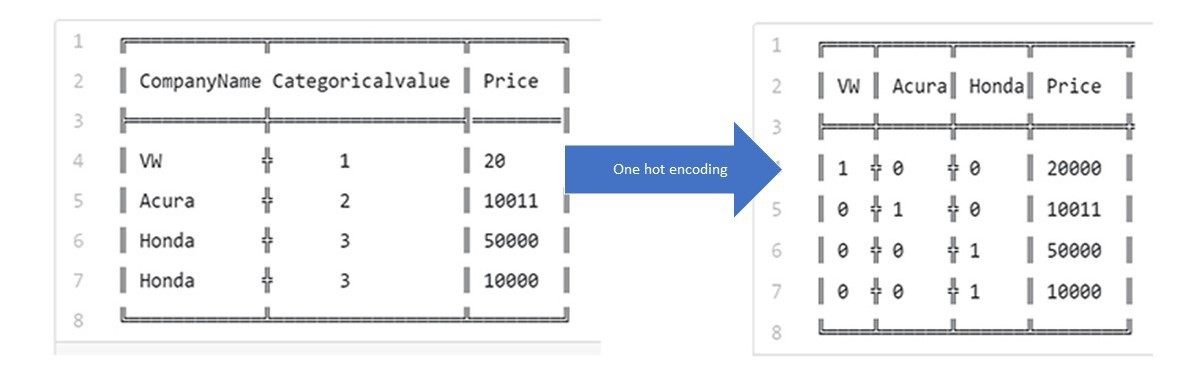
\includegraphics[width=\textwidth]{./Figure/onehotexample.png}
    \caption{One hot encoding explained in an image.}
    \label{fig:onehotexample}
\end{figure}

\subsection{Prediction of malware}

After preprocessing our data to the best format for all of our classifiers, finally, we do the malware prediction step.
We input the preprocessed data to the 49 models as mentioned in section \ref{model}.
After the 3 steps of prediction, the final classifier outputs the final prediction (0 for Benign app, 1 for Malware app).

